\documentclass[12pt]{article}
\usepackage[T2A]{fontenc}
\usepackage[russian, english]{babel}
\usepackage[utf8x]{inputenc}
\usepackage{amsmath, amssymb}
\usepackage{graphicx}
\usepackage{physics}
\usepackage{float}
\usepackage{booktabs} 
\usepackage{amsmath}
\usepackage{systeme}
\usepackage{blindtext}
\usepackage{enumitem}
\usepackage{listings}
\usepackage[table]{xcolor}
\usepackage{hyperref}
\usepackage{tikz}
\usepackage{titlesec}
\usepackage{mathtools}
\usepackage{tcolorbox}
\usepackage{bm}
\usepackage[normalem]{ulem}
\usepackage{geometry}
\usepackage{siunitx}
\usepackage{xcolor}
\usepackage{tikzsymbols}
\usepackage{relsize}
\usepackage{pgfplots}
\usepackage[edges]{forest}
\usepackage{minted}
\usepackage{csquotes}
\usepackage{pgfplots}
\usepackage{color}
\usepackage{textcomp}
\usepackage{subcaption}

\geometry{
    a4paper,
    left=2cm,
    right=2cm,
    top=1.5cm,
    bottom=1.5cm
}
\usepackage{multicol}

\usemintedstyle{emacs}

\setminted[cpp]{ %
    linenos=true,             % Line numbers
    autogobble=true,          % Automatically remove common white space
    frame=lines,
    framesep=2mm,
    fontsize=\footnotesize,
}

\makeatletter
\newenvironment{code}
 {\RecustomVerbatimEnvironment{Verbatim}{BVerbatim}{}%
  \def\FV@BProcessLine##1{%
    \hbox{%
      \hbox to\z@{\hss\theFancyVerbLine\kern\FV@NumberSep}%
      \FancyVerbFormatLine{##1}%
    }%
  }%
  \VerbatimEnvironment
  \setbox\z@=\hbox\bgroup
  \begin{minted}{cpp}}
 {\end{minted}\egroup
  \leavevmode\vbox{\hrule\kern2mm\box\z@\kern2mm\hrule}}
\makeatother

\definecolor{mintedbackground}{rgb}{0.95,0.95,0.95}

\newmintedfile[cmakecode]{cmake}{
bgcolor=mintedbackground,
fontfamily=tt,
linenos=true,
numberblanklines=true,
numbersep=5pt,
gobble=0,
frame=leftline,
framerule=0.4pt,
framesep=2mm,
funcnamehighlighting=true,
tabsize=4,
obeytabs=false,
mathescape=false
samepage=false, %with this setting you can force the list to appear on the same page
showspaces=false,
showtabs =false,
texcl=false,
}

\definecolor{mygray}{rgb}{0.4,0.4,0.4}
\definecolor{mygreen}{rgb}{0,0.8,0.6}
\definecolor{myorange}{rgb}{1.0,0.4,0}

\lstset{
basicstyle=\footnotesize\sffamily\color{black},
commentstyle=\color{mygray},
frame=single,
numbers=left,
numbersep=5pt,
numberstyle=\tiny\color{mygray},
keywordstyle=\color{mygreen},
showspaces=false,
showstringspaces=false,
stringstyle=\color{myorange},
tabsize=2
}

\pgfmathdeclarefunction{gauss}{2}{\pgfmathparse{1/(#2*sqrt(2*pi))*exp(-((x-#1)^2)/(2*#2^2))}}

\DeclareRobustCommand{\bbone}{\text{\usefont{U}{bbold}{m}{n}1}}

\DeclareMathOperator{\EX}{\mathbb{E}}

\newcommand{\icol}[1]{% inline column vector
  \left[\begin{smallmatrix}#1\end{smallmatrix}\right]%
}


\titleclass{\subsubsubsection}{straight}[\subsection]

\newcounter{subsubsubsection}[subsubsection]
\renewcommand\thesubsubsubsection{\thesubsubsection.\arabic{subsubsubsection}}
\renewcommand\theparagraph{\thesubsubsubsection.\arabic{paragraph}} % optional; useful if paragraphs are to be numbered

% Set paragraph indent
\setlength{\parindent}{4ex}

% Set the header of the ToC as "Оглавление"
\addto\captionsenglish{
  \renewcommand{\contentsname}
    {Оглавление}
}

\titleformat{\subsubsubsection}
  {\normalfont\normalsize\bfseries}{\thesubsubsubsection}{1em}{}
\titlespacing*{\subsubsubsection}
{0pt}{3.25ex plus 1ex minus .2ex}{1.5ex plus .2ex}

\makeatletter
\renewcommand\paragraph{\@startsection{paragraph}{5}{\z@}%
  {3.25ex \@plus1ex \@minus.2ex}%
  {-1em}%
  {\normalfont\normalsize\bfseries}}
\renewcommand\subparagraph{\@startsection{subparagraph}{6}{\parindent}%
  {3.25ex \@plus1ex \@minus .2ex}%
  {-1em}%
  {\normalfont\normalsize\bfseries}}
\def\toclevel@subsubsubsection{4}
\def\toclevel@paragraph{5}
\def\toclevel@paragraph{6}
\def\l@subsubsubsection{\@dottedtocline{4}{7em}{4em}}
\def\l@paragraph{\@dottedtocline{5}{10em}{5em}}
\def\l@subparagraph{\@dottedtocline{6}{14em}{6em}}
\makeatother

\setcounter{secnumdepth}{4}
\setcounter{tocdepth}{4}

\hypersetup{
	colorlinks=true,
    linkcolor=blue,
    filecolor=magenta,      
    urlcolor=cyan,
}

\definecolor{codegreen}{rgb}{0,0.6,0}
\definecolor{codegray}{rgb}{0.5,0.5,0.5}
\definecolor{codepurple}{rgb}{0.58,0,0.82}
\definecolor{backcolour}{rgb}{0.95,0.95,0.92}

\lstdefinestyle{mystyle}{
    backgroundcolor=\color{backcolour},   
    commentstyle=\color{codegreen},
    keywordstyle=\color{magenta},
    numberstyle=\tiny\color{codegray},
    stringstyle=\color{codepurple},
    basicstyle=\ttfamily\footnotesize,
    breakatwhitespace=false,         
    breaklines=true,                 
    captionpos=b,                    
    keepspaces=true,                 
    numbers=left,                    
    numbersep=5pt,                  
    showspaces=false,                
    showstringspaces=false,
    showtabs=false,                  
    tabsize=2
}

\pagenumbering{arabic}

\begin{document}
    \begin{titlepage}
    \center % Center everything on the page
    \newcommand{\HRline}[1]{\rule{\linewidth}{#1}} % Defines a new command for the horizontal lines, change thickness here
    %----------------------------------------------------------------------------------------
    %	HEADING SECTIONS
    %----------------------------------------------------------------------------------------

    
\includegraphics[scale=1]{images/logo.jpg}\\[1cm] % Include a department/university logo - this will require the graphicx package
    \textbf{\large МИНОБРНАУКИ РОССИИ}\\[0.5cm]
    \textbf{\large федеральное государственное бюджетное образовательное учреждение}\\[0.2cm]
    \textbf{\large высшего образования}\\[0.2cm]
    \textbf{\large <<Московский государственный технологический университет}\\[0.2cm]
    \textbf{<<СТАНКИН>>}\\[0.5cm]

    \textbf{\large (ФГБОУ ВО «МГТУ «СТАНКИН»)}
    \HRline{0.02cm} \\[0.1cm]

    \begin{multicols}{2}
        \begin{flushleft}
            \textbf{\large Институт}\\
            \textbf{\large информационных}\\
            \textbf{\large систем и технологий}\\
        \end{flushleft}
        
        \columnbreak
        \begin{flushleft}
            \textbf{\large Кафедра}\\
            \textbf{\large информационных систем}\\
        \end{flushleft}

    \end{multicols}

    %----------------------------------------------------------------------------------------
    %	TITLE SECTION
    %----------------------------------------------------------------------------------------
    \textbf{\large Программирование специализированных вычислительных устройств}\\
    \textbf{\large Отчет по лабораторной работе}\\[0.5cm]


    { \Large \bfseries <<3D моделлирование посредством OpenGL для Веба>> Часть \textnumero 1}\\ % Title of your document
    \HRline{0.02cm} \\[1.5cm]
    
    %----------------------------------------------------------------------------------------
    %	AUTHOR SECTION
    %----------------------------------------------------------------------------------------

    \begin{minipage}{\textwidth}
    \begin{multicols}{2}
        \begin{flushleft}
            \large Студент группы ИДБ-19-07:\\
            \large Проверил доцент кафедры ИС:
        \end{flushleft}

        
        \columnbreak
        \begin{flushright}
            \large Касьян А.И.\\
            \large к.т.н. Волкова О.Р.
        \end{flushright}

    \end{multicols}

    \end{minipage}\\[8cm]

    % If you don't want a supervisor, uncomment the two lines below and remove the section above
    %\Large \emph{Author:}\\
    %John \textsc{Smith}\\[3cm] % Your name

    %----------------------------------------------------------------------------------------
    %	DATE SECTION
    %----------------------------------------------------------------------------------------

    {\large \today}\\[2cm] % Date, change the \today to a set date if you want to be precise


    \end{titlepage}

    \newpage

    \tableofcontents

    \newpage

    \section{Вводное слово}
    В данной секции я бы хотел обозначить некоторые моменты, которые могут
    сбивать.
    \begin{itemize}
        \item Данный, как и все остальные документы я оформляю с помощью 
        LaTex, в связи с этим ни doc ни docx файлы предоставить не могу 
        (если таковые потребуются). Все source-файлы находятся на 
        \href{https://github.com/JuiceFV/Emscripten_OpenGL}{GitHub'е}
        в соответствующей папке \emph{\href{https://github.com/JuiceFV/Emscripten_OpenGL/tree/master/doc}{doc}}
        \item Из-за не маленького количества кода я не могу полностью сопроводить листингом.
        Весь код есть на моём \href{https://github.com/JuiceFV/Emscripten_OpenGL}{GitHub'е}.
        Однако, основные моменты я вставлю и прокоментирую.
        \item Всвязи с плотным графиком на работе, я не могу уделять время на лаб. работы.
        По этой же причине я взял задание у преподавателя ООП (Разумовского А.И.)
        и оно по своей тематике очень схоже с лаб. работами.
        \item Я сразу хочу подметить, что проект не создавался как кроссплатформенное
        решение, т.к. я считаю, что это глупо использовать для кроссплатформы
        OpenGL (так считаю не только я: \href{https://www.youtube.com/watch?v=W3gAzLwfIP0}{ссылка на видео}), т.к. у каждой платформы есть более подходящие спецификации, с 
        более комплексным и гибким API. Поэтому проект работает на
        платформе Windows (а точнее, компилятор MSVC) и Windows/*nix 
        с компилятором emcc (\href{https://emscripten.org/}{Emscripten compiler}).
        За поведение при использовании других компиляторов я ответственности не 
        несу.
        \item Если вы заглянете в код, коментарии там на английском. Т.к.
        я в большинстве случаев использую английский и мне на нём проще 
        излагать свои мысли. (Если взгляните на мой GH, он весь на английском).
    \end{itemize}
    \newpage
    \section{Постановка задания}
    Требуется реализовать отрисовку 3D-моделей, посредством OpenGL и портировать программу
    под web, с помощью \href{https://emscripten.org/}{Emscripten}. Так же должна 
    присутствовать возможность осмотра модели, я это сделал посредством камеры, 
    сама модель статична. В идеале результат должен выглядеть как-то так:

    \begin{figure}[!h]
        \begin{subfigure}{.5\textwidth}
          \centering
          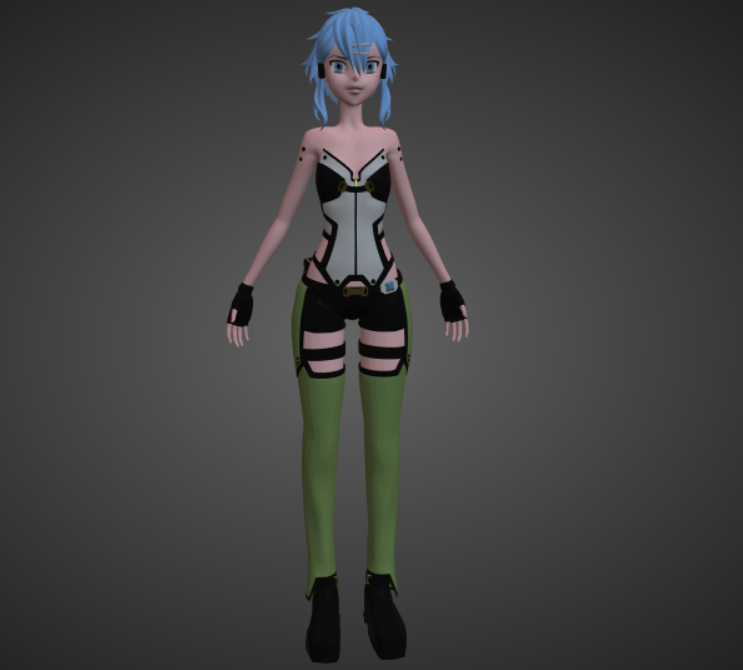
\includegraphics[width=.8\linewidth]{images/front.png}
          \caption{front}
          \label{fig:sfig1}
        \end{subfigure}%
        \begin{subfigure}{.5\textwidth}
          \centering
          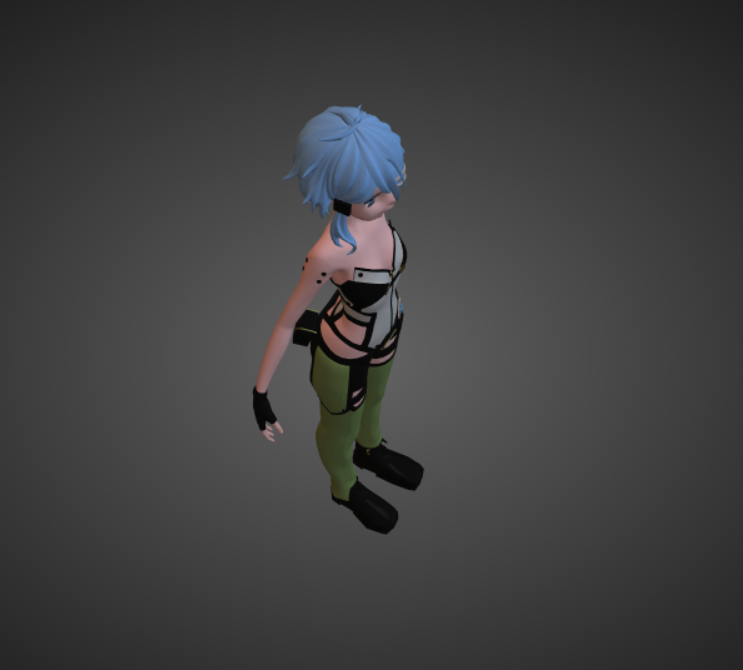
\includegraphics[width=.8\linewidth]{images/Rotation.png}
          \caption{rotation}
          \label{fig:sfig2}
        \end{subfigure}
        \\
        \begin{subfigure}{.5\textwidth}
            \centering
            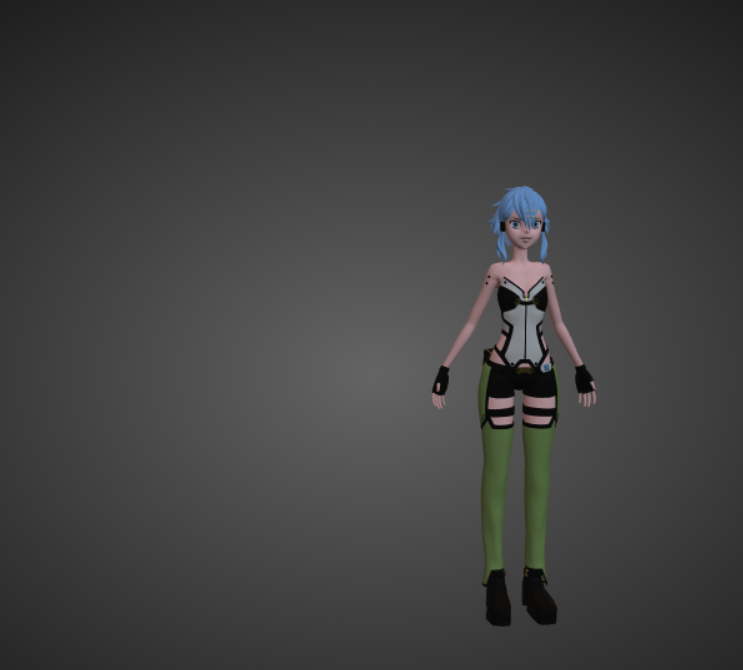
\includegraphics[width=.8\linewidth]{images/movement.png}
            \caption{movement}
            \label{fig:sfig2}
          \end{subfigure}
          \begin{subfigure}{.5\textwidth}
            \centering
            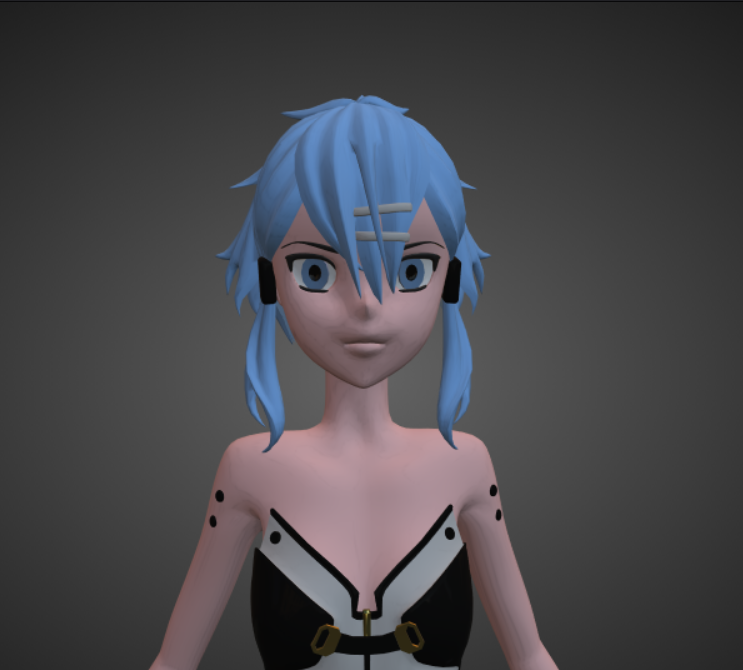
\includegraphics[width=.8\linewidth]{images/zoom.png}
            \caption{zoom}
            \label{fig:sfig2}
          \end{subfigure}
        \caption{Transformations}
        \label{fig:fig}
    \end{figure}
    \section{Набор инструментов}
    \begin{enumerate}
        \item \href{https://www.docker.com/}{Docker} - для развёртки на любой машине
        \item \href{https://ci.appveyor.com/project/JuiceFV/emscripten-opengl/}{Appveyor} - сборка и тестирование для MSVC компиляторов
        \item \href{https://travis-ci.org/github/JuiceFV/Emscripten_OpenGL}{Travis} - сборка и тестирование для emscripten.
        \item \href{https://cmake.org/}{CMake} - для генерации файлов сборки.
        \item \href{https://github.com/google/googletest}{googletests} - для тестов.
        \item \href{https://www.python.org/}{Python3} - для запуска вебсервера
        \item \href{https://github.com/jbeder/yaml-cpp}{YAML-CPP 0.6.3} - для парсинга YAML файлов
        \item \href{https://github.com/glfw/glfw/releases/tag/3.3.2}{GLFW 3.3.2} - API для OpenGL.
        \item \href{https://github.com/nigels-com/glew/releases/tag/glew-2.1.0}{GLEW 2.1.0} - для низкоуровневого взаимодействия с OpenGL.
        \item \href{https://github.com/SpartanJ/SOIL2/releases/tag/release-1.20}{SOIL 1.20} - библиотека для загрузки изображений.
        \item \href{https://github.com/g-truc/glm/releases/tag/0.9.9.8}{GLM 0.9.9.8} - библиотека для удобной работы с линейной алгеброй и OpenGL.
        \item \href{https://github.com/emscripten-core/emsdk/releases/tag/2.0.7}{EMSDK 2.0.7} - emscripten compiler.
        \item \href{https://github.com/assimp/assimp/releases/tag/v5.0.1}{Assimp 5.0.1} - для парсинга obj и mlt файлов.
    \end{enumerate}
    \section{Результат выполнения задания}
    В данной части я распишу принцип работы шейдоров и класс, который я создал
    (будем честными, нагло скопипастил и разобрал). А в следующей я разберу 
    трансформации и текстуры.

    \subsection{CMake}
    Начну я с CMake'a, т.к. это одна из основопологающих проекта.
    Так как я пишу под разные компиляторы - я использую генерацию сборочных файлов.
    Поэтому я думаю стоит уделить пару слов CMakeLists.txt.

    \cmakecode{cmakes/setsrc.txt}
    Технически, в данном куске мы собираем все файлы, требуемые для проекта.
    Далее я подключаю созданные мною модули, которые лежат в \emph{\href{https://github.com/JuiceFV/Emscripten_OpenGL/tree/master/cmake/Modules}{cmake/Modules}}

    \cmakecode{cmakes/modules.txt}
    Я думаю стоит пробежаться только по двум модулям - graphics и configloader.
    \begin{enumerate}
        \item Дабы сделать интерфейс более удобным, я добавил конфигурацию проекта
        через yaml-файл. И написал небольшую библиотеку для чтения конфигурационного файла.
        В configloader находится сборка данной библиотеки. По данному пути \emph{\href{https://github.com/JuiceFV/Emscripten_OpenGL/blob/master/application/configloader/CMakeLists.txt}{application/configloader/CMakeLists.txt}}
        вы можете найти CMakeList, который собирает эту библиотеку из source-файлов.
        \item graphics в свою очередь собирает и устанавливает флаги линковки для графических
        библиотек. В связи с тем, что у Emscripten есть свой GLFW, там стоят пару if-else, в зависимости от компиляторов.
    \end{enumerate}
    \noindent
    Далее устанавливаются листы с библиотеками:

    \cmakecode{cmakes/setlibs.txt}
    Библиотеки разделены на несколько групп, т.к. для Emscripten'a
    не требуется API для OpenGL, да и OpenGL как токовой (веб использует
    WebGL =/). А у glm интерфейссное подключения, а т.к. я преношу все библиотеки
    в одно место при генерации сборочных файлов - перенести glm не удасться.
    
    \noindent
    Создаём исполняемый файл и линкуем все библиотеки к нему. Некоторые библиотеки
    линкуются, только если компилятор - это MSVC. 

    \cmakecode{cmakes/exe.txt}

    \subsection{Шейдеры}
    Как я и говорил в этой части я разберу только шейдеры.
    Т.к. я использую веб версию, которая не поддерживает GLSL 
    пришлось шейдеры разделить на отдельные группы файлов (для десктопа и для веба).
    Но выглядят они очень схоже:
    \begin{figure}[!h]
        \begin{subfigure}{.6\textwidth}
          \begin{code}
#version 330 core


in vec2 TexCoord;

out vec4 color;

uniform sampler2D ourTexture1;

void main()
{
    color = texture(ourTexture1, TexCoord);
}
          \end{code}
          \caption{desktop fragment shader}
          \label{fig:sfig1}
        \end{subfigure}%
        \begin{subfigure}{.6\textwidth}
          \begin{code}
#version 300 es
precision mediump float;

in vec2 TexCoord;

out vec4 color;

uniform sampler2D ourTexture1;

void main()
{
    color = texture(ourTexture1, TexCoord);
}
          \end{code}
          \caption{web fragment shader}
          \label{fig:sfig2}
        \end{subfigure}
        \\
        \begin{subfigure}{.6\textwidth}
            \begin{code}
#version 330 core
layout (location = 0) in vec3 position;
layout (location = 2) in vec2 texCoord;
out vec2 TexCoord;
uniform mat4 model;
uniform mat4 view;
uniform mat4 projection;

void main()
{
    gl_Position = projection * view * model
         * vec4(position, 1.0f);

    TexCoord = vec2(texCoord.x, 
                    1.0 - texCoord.y);
}
            \end{code}
            \caption{vertex shader}
            \label{fig:sfig2}
          \end{subfigure}
          \begin{subfigure}{.6\textwidth}
            \begin{code}
#version 300 es
layout (location = 0) in vec3 position;
layout (location = 2) in vec2 texCoord;
out vec2 TexCoord;
uniform mat4 model;
uniform mat4 view;
uniform mat4 projection;

void main()
{
    gl_Position = projection * view * model 
                    * vec4(position, 1.0f);

    TexCoord = vec2(texCoord.x, 
                1.0 - texCoord.y);
}
            \end{code}
            \caption{web vertex shader}
            \label{fig:sfig2}
          \end{subfigure}
        \caption{Shaders}
        \label{fig:fig}
    \end{figure}
    \newpage
    \noindent
    Я разделил шейдеры на файлы с соответсвующими расширениями:
    \begin{itemize}
        \item \textbf{vs} - вертекс шейдеры
        \item \textbf{frag} - фрагмент шейдеры
        \item \textbf{wvs} - вертекс шейдеры для веба
        \item \textbf{wfrag} - фрагмент шейдеры для веба
    \end{itemize}
    Код шейдера я разбирать не хочу, он максимально тревиален и скопирован
    из первого попавшегося туториала. В вертекс шейдере на вход принимается
    координата текстуры, на выходе ловим цвет этой координты, согласно глобально-
    установленной текстуре. Во фрагмент шейдере на входе передаётся позиция
    и кордината текстуры, так же присутствуют матрицы, отвечающие за трансформацию.
    Устанавливаем позицию и координату текстуры.

    \subsection{Обработка шейдеров}
    Для обработки шейдеров я создал класс Shader, его интерфейс выглядит так:
    \begin{figure}[!htb]
        \centering
        \begin{code}
class Shader
{
  private:
    // Member vars
    unsigned int program;
    std::string loadShaderFile(const char *path);
    unsigned int compileShader(unsigned int type, const char *path);
    void linkProgram(unsigned int vertex_shader, unsigned int fragment_shader);
  public:
    // Constructor generates the shader on the fly
    Shader(const char *vertex_path, const char *fragment_path);
    // Uses the current shader
    void Use();
    void Unuse();
    void set1i(int value, const char *name);
    void setMat4fv(glm::mat4 value, const char *name, unsigned char transpose = GL_FALSE);
    ~Shader();
};
        \end{code}
        \caption{Shaders Interface}
    \end{figure}\\
    \noindent
    Я не хочу приводить листинг всей имплиментации - с ней можно ознакомиться
    на \href{https://github.com/JuiceFV/Emscripten_OpenGL}{GitHub'е}. Я приведу
    только те, которые мне кажется стоят пояснения. Дабы не загряхнять код 
    в основном файле - я вынес установку матриц (на данный момент для трансформации)
    в отдельные методы. 
    \begin{figure}[!htb]
        \begin{code}
    void Shader::set1i(int value, const char *name)
    {
        this->Use();
        glUniform1i(glGetUniformLocation(this->program, name), value);
        this->Unuse();
    }
    void Shader::setMat4fv(glm::mat4 value, const char *name, unsigned char transpose)
    {
        this->Use();
        glUniformMatrix4fv(glGetUniformLocation(this->program, name), 1, transpose, glm::value_ptr(value));
        this->Unuse();
    }
        \end{code}
    \end{figure}
    
    \begin{figure}[!htb]
        \centering
        \begin{code}
std::string Shader::loadShaderFile(const char *path)
{
    std::string shader_code;   // The code of shaders as a string
    std::ifstream shader_file; // The very file
    // ensures ifstream objects able to throw exceptions
    shader_file.exceptions(std::ifstream::badbit);
    try
    {
        // Open file
        shader_file.open(path);
        std::stringstream shader_stream;
        // Read file's buffer contents into stream
        shader_stream << shader_file.rdbuf();
        // close file handler
        shader_file.close();
        // Convert stream into string
        shader_code = shader_stream.str();
    }
    catch (std::ifstream::failure &error)
    {
        std::cerr << "An error has occured in the " << __FILE__ 
                  << " in line " << __LINE__ << "." << std::endl
                  << "Details: " << error.what() << std::endl;
    }
    return (shader_code);
}

unsigned int Shader::compileShader(unsigned int type, const char *path)
{
    char log_info[512]; // log information if something wrong
    int success;        // the variable indicates if a shader's compilation went wrong

    // shader of a specific type (vertex/fragment/geometry)
    unsigned int shader = glCreateShader(type);
    // load source code from a file
    std::string str_shader_code = loadShaderFile(path);
    const char *shader_code = str_shader_code.c_str();
    // compile shaders itself
    glShaderSource(shader, 1, &shader_code, NULL);
    glCompileShader(shader);

    // check if a compilation done well
    glGetShaderiv(shader, GL_COMPILE_STATUS, &success);
    if (!success)
    {
        glGetShaderInfoLog(shader, 512, NULL, log_info);
        std::cerr << "An error has occured in the " << __FILE__ 
                  << " in line " << __LINE__ << "." << std::endl
                  << "Error occured in the: " << path << std::endl
                  << "Details: " << log_info << std::endl;
    }
    return shader;
}
        \end{code}
        \caption{Shaders Interface}
    \end{figure}
    \noindent
    Все пояснения хорошо оформлены мной в коментариях.
    \subsection{Использование шейдеров}
    На данный момент я их использую в основном файле, потом это занесётся в отдельный
    класс. Я заменил код, который не относится к шейдерам на <<...>> дабы не громоздить здесь.

        \begin{code}
int main()
{
    ...
#ifndef __EMSCRIPTEN__
    Shader ourShader("assets/shaders/core.vs", "assets/shaders/core.frag");
#else
    Shader ourShader("assets/shaders/core.wvs", "assets/shaders/core.wfrag");
#endif
    ...
#ifdef __EMSCRIPTEN__
    std::function<void()> mainLoop = [&]() {
#else
    while (!glfwWindowShouldClose(window))
    {
#endif
        // Set frame time
        ...
        // Check and call events
        ...
        // Clear the colorbuffer
        ...
        // Draw our first triangle
        ourShader.Use();

        // Bind Textures using texture units
        texture.bind(0);
        ourShader.set1i(0, "ourTexture1");

        glm::mat4 projection(1);
        projection = glm::perspective(camera.GetZoom(), 
                     (GLfloat)SCREEN_WIDTH / (GLfloat)SCREEN_HEIGHT, 
                     0.1f, 1000.0f);

        // Create camera transformation
        glm::mat4 view(1);
        view = camera.GetViewMatrix();

        // Pass the matrices to the shader
        ourShader.setMat4fv(view, "view");
        ourShader.setMat4fv(projection, "projection");

        glBindVertexArray(VAO);

        for (GLuint i = 0; i < 10; i++)
        {
            // Calculate the model matrix for each object and pass it to shader before drawing
            ourShader.setMat4fv(model, "model");
            ourShader.Use();
            glDrawArrays(GL_TRIANGLES, 0, 36);
        }

        glBindVertexArray(0);

        // Swap the buffers
        glfwSwapBuffers(window);
#ifdef __EMSCRIPTEN__
    };
    emscripten_set_main_loop_arg(dispatch_main, &mainLoop, 0, 1);
#else
    }
#endif
...
}
        \end{code}

    \newpage
    \noindent
    Небольшой момент, который я пояснию - это компиляционные дерективы \texttt{ifdef-else-endif}
    Т.к. для emscripten'a требуется немного другой синтаксис - для этого я использую компиляционные
    дерективы \texttt{ifdef-else-endif}, которые в зависимоти от компилятора будут подгружать
    разные файлы с шейдерами.
    \section{Промежуточный результат}
    В данном документе я показываю, что шейдеры работают правильно.
    Т.е. то, что отображается и как - на данном этапе нас не волнует.

    \begin{figure}[!h]
        \centering
        \begin{subfigure}{.9\textwidth}
          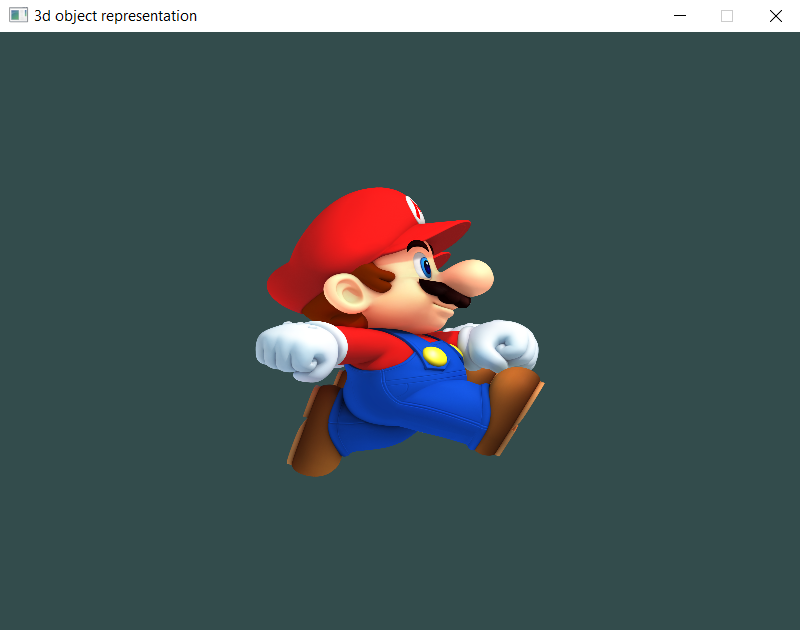
\includegraphics[width=\linewidth]{images/shaders_result.png}
          \caption{Shader's proper result}
          \label{fig:sfig1}
        \end{subfigure}%
    \end{figure}
    \section{Конец первой части}
    На этом я закончу небольшой разбор шейдеров и их обработку.
    Во второй части мы рассмотрим:
    \begin{itemize}
        \item Трансформацию и текстурирование.
        \item Так же я уделю немного места для emscripten'a. 
        \item Посмотрим на результат, который у меня имеется на 
        данный момент.
        \item Затронем что ещё необходимо сделать/улучшить.
    \end{itemize}
    
\end{document}